\documentclass[acmtog]{acmart}
\usepackage{graphicx}
\usepackage{subfigure}
\usepackage{natbib}
\usepackage{listings}
\usepackage{bm}
\usepackage{amsmath}

\definecolor{mygreen}{rgb}{0,0.6,0}
\definecolor{mygray}{rgb}{0.5,0.5,0.5}
\definecolor{mymauve}{rgb}{0.58,0,0.82}
\lstset{ %
backgroundcolor=\color{white},   % choose the background color
basicstyle=\footnotesize\ttfamily,        % size of fonts used for the code
columns=fullflexible,
breaklines=true,                 % automatic line breaking only at whitespace
captionpos=b,                    % sets the caption-position to bottom
tabsize=4,
commentstyle=\color{mygreen},    % comment style
escapeinside={\%*}{*)},          % if you want to add LaTeX within your code
keywordstyle=\color{blue},       % keyword style
stringstyle=\color{mymauve}\ttfamily,     % string literal style
frame=single,
rulesepcolor=\color{red!20!green!20!blue!20},
% identifierstyle=\color{red},
language=c++,
}


\definecolor{blve}{rgb}{0.3372549 , 0.61176471, 0.83921569}
\definecolor{gr33n}{rgb}{0.29019608, 0.7372549, 0.64705882}
\makeatletter
\lst@InstallKeywords k{class}{classstyle}\slshape{classstyle}{}ld
\makeatother
\lstset{language=C++,
	basicstyle=\ttfamily,
	keywordstyle=\color{blve}\ttfamily,
	stringstyle=\color{red}\ttfamily,
	commentstyle=\color{magenta}\ttfamily,
	morecomment=[l][\color{magenta}]{\#},
	classstyle = \bfseries\color{gr33n}, 
	tabsize=2
}
\lstset{basicstyle=\ttfamily}

% Title portion
\title{Assignment 3: {Ray Tracing Basics}} 

\author{Name:\quad Entropy-Fighter\\ student number:\ 2020533
\\email:\quad xxxx@shanghaitech.edu.cn}

% Document starts
\begin{document}
\maketitle

\vspace*{2 ex}

\section{Introduction}
\quad I do the must, bonus1, bonus2 and bonus4.
\begin{itemize}
\item (must)generate rays from camera (10 pts)
\item (must)ray geometry intersection (30 pts)
\item (must)Phong lighting at intersection (15 pts)
\item (must)light ray sampling for soft shadow (25 pts)
\item (must)anti-aliasing by super-resolution (10 pts)
\item (optional)texture mapping (10 pts)
\item (optional)normal/displacement texture (15 pts)
\item (optional)advanced anti-aliasing (10 pts)
\end{itemize}



\section{Implementation Details}

\subsection{Construct a virtual Camera}
\quad This part is implemented in the "camera.cpp".
In order to construct a virtual camera, we need to know the resolution, height, weight, the world position, the field of view, the focal lenght.

Also, it is important to get the lookat matrix. 
It is implemented in "lookat" function. The forward direction is calculated based on the "lookat coordinate" and the camera position. 
Then we calculate the right direction by the cross product of calculated forward direction and ref\_up direction. 
At last, the up direction is calculated by the cross product of right direction and forward direction.

\subsection{Generate Rays From Camera}
\quad This part is implemented in the "camera.cpp". 
This part is illustrated clearly in the tutorial6, first, let us see 2 pictures. 
\begin{figure}[h]
	\centering
	{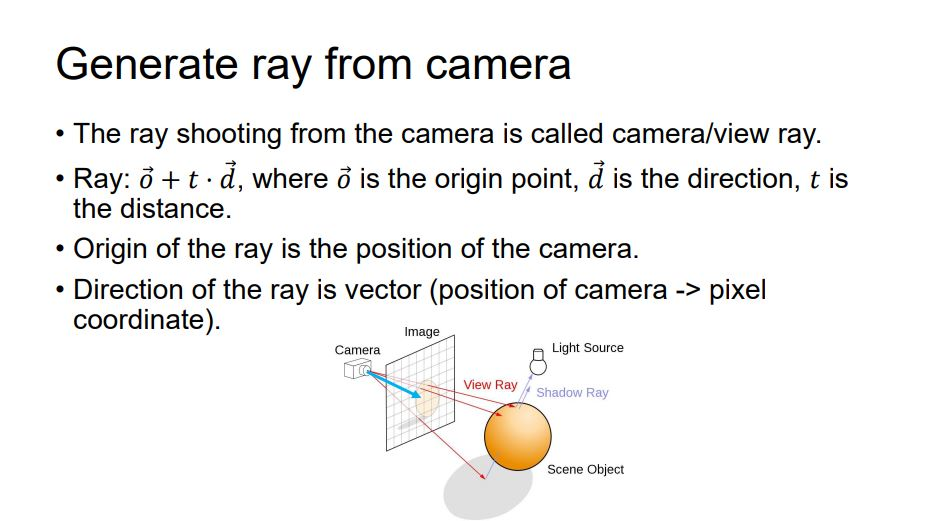
\includegraphics[width=8cm]{c1.JPG}}	
\end{figure}

\begin{figure}[h]
	\centering
	{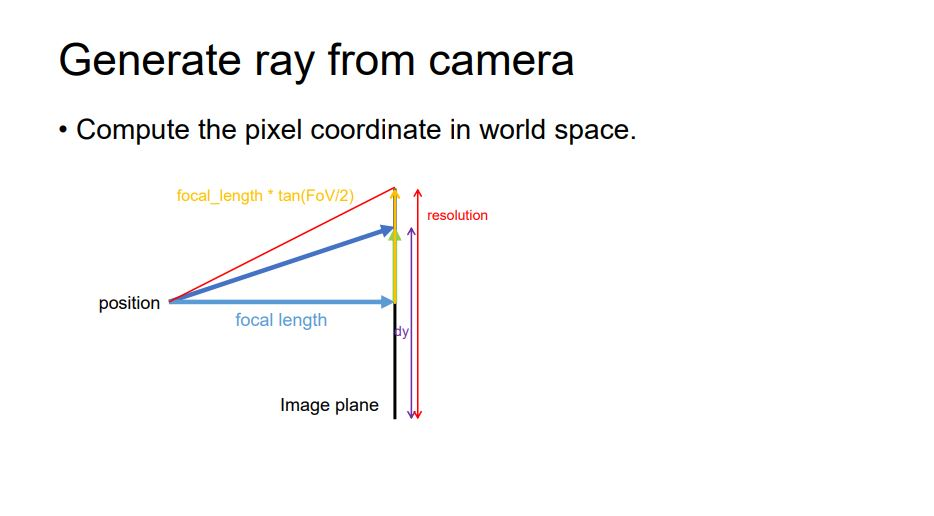
\includegraphics[width=8cm]{c2.JPG}}	
\end{figure}
In order to get a ray from the camera, we have "dx" and "dy" as input parameters but we need the world coordinates.

Firstly we should normalize the dx and dy, where (0, 0) is the orgin. After that, we have some small tricks to transform these coordinates to screen coordinates. 
The small tricks to transform to the screen coordinates can be easily knowned from the figure 2 above.

Then, we use the formula: "position = screenCenter + screen\_x * right + screen\_y * up" to get world position, use formula: "(position - this->position).normalized()" to get direction.


At last, The ray can be easily discribed as O + t * d.


\subsection{Ray Geometry Intersection}

\quad This part is implemented in the "geometry.cpp". 
There are 3 types of geometries: triangle, rectangle and ellipsoid.

As for triangles, the class ppt gives us a quick solution. The concrete steps can be seen in pictures bellow. 
Although the matrix calculation is complex, we just use the conclusion in slides to code.

% \begin{figure}[h]
% 	\centering
% 	{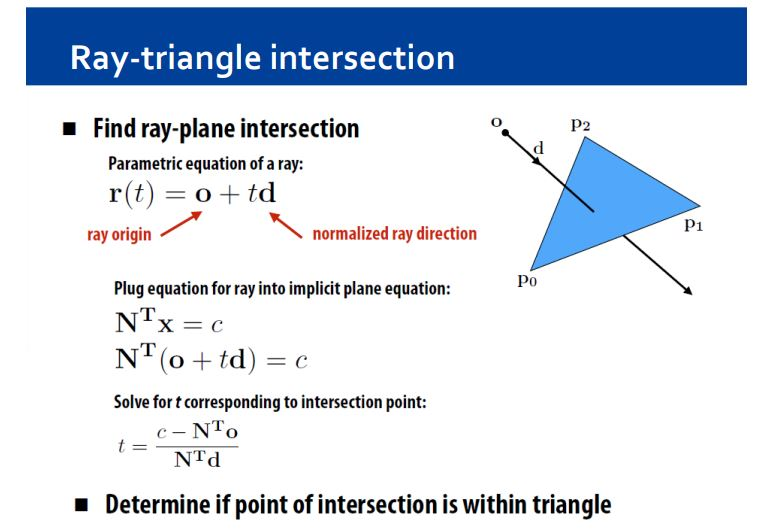
\includegraphics[width=8cm]{t1.JPG}}	
% \end{figure}
% \begin{figure}[h]
% 	\centering
% 	{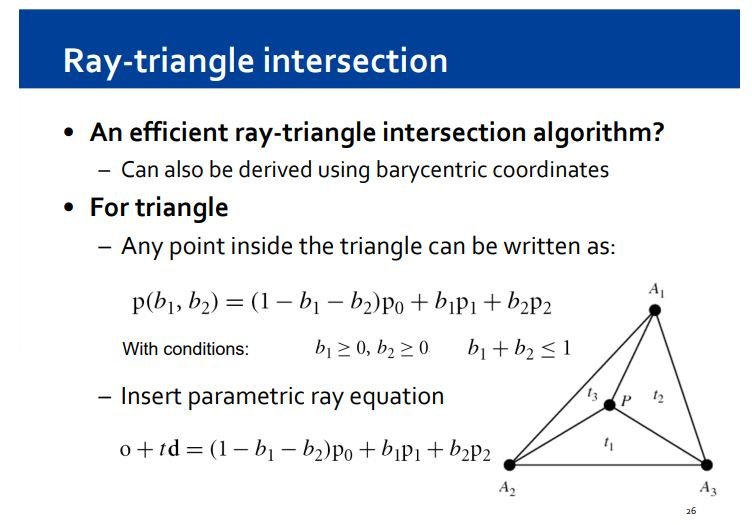
\includegraphics[width=8cm]{t2.JPG}}	
% \end{figure}
% \begin{figure}[h]
% 	\centering
% 	{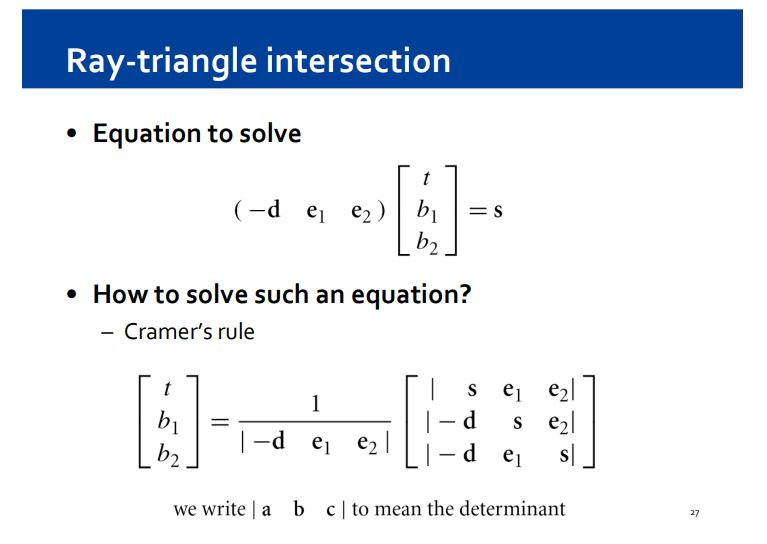
\includegraphics[width=8cm]{t3.JPG}}	
% \end{figure}
% \begin{figure}[h]
% 	\centering
% 	{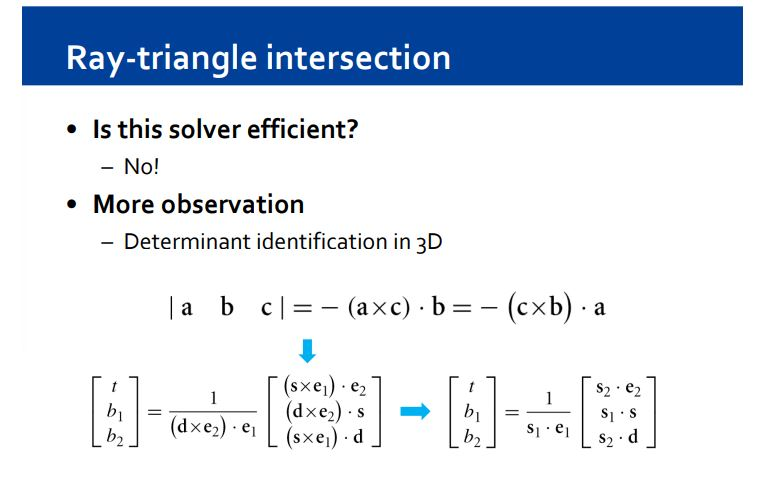
\includegraphics[width=8cm]{t4.JPG}}	
% \end{figure}

\begin{figure}[h]
    \centering
    \subfigure[]
    {
        \begin{minipage}[b]{.4\linewidth}
            \centering
            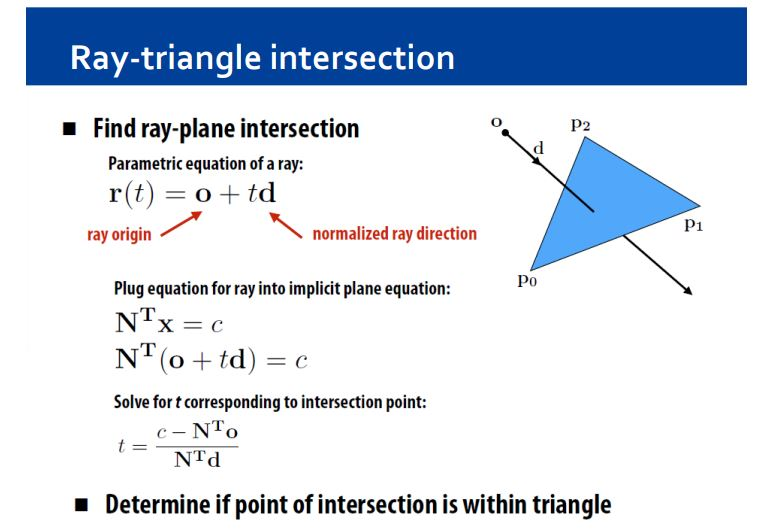
\includegraphics[scale=0.25]{t1.JPG}
        \end{minipage}
    }
    \subfigure[]
    {
        \begin{minipage}[b]{.4\linewidth}
            \centering
            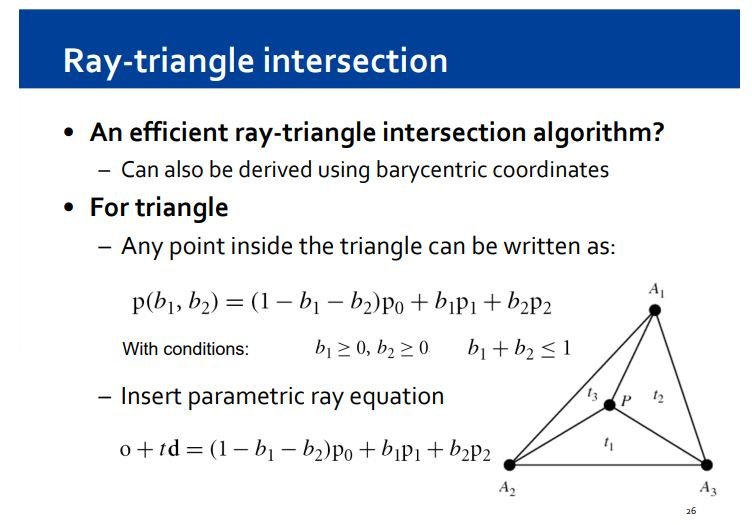
\includegraphics[scale=0.25]{t2.JPG}
        \end{minipage}
    }
    \\
    \subfigure[] 
    {
        \begin{minipage}[b]{.4\linewidth}
            \centering
            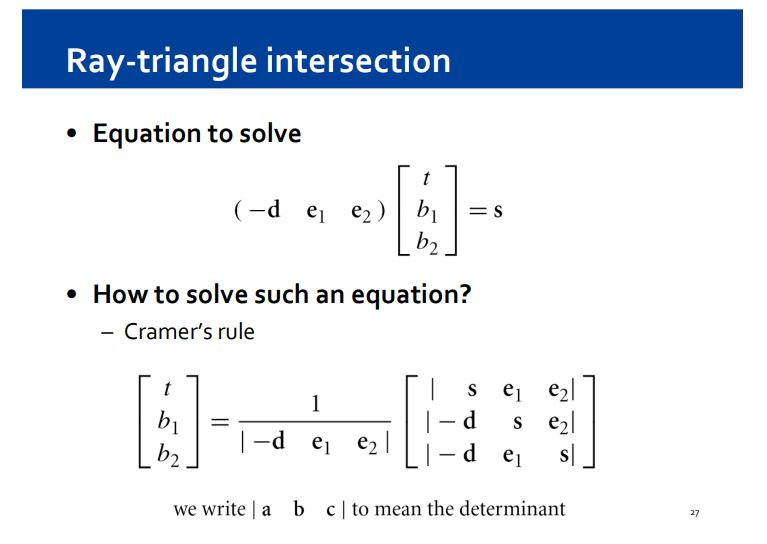
\includegraphics[scale=0.25]{t3.JPG}
        \end{minipage}
    }
    \subfigure[]
    {
        \begin{minipage}[b]{.4\linewidth}
            \centering
            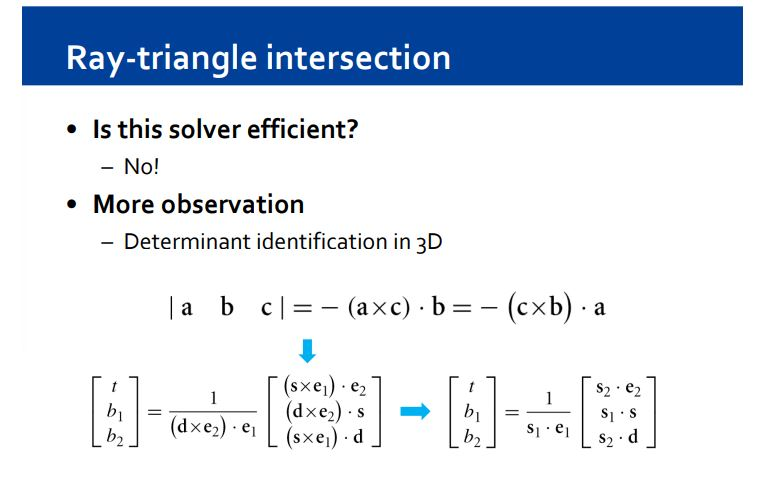
\includegraphics[scale=0.25]{t4.JPG}
        \end{minipage}
    }
    \caption{Triangle interseciton}
\end{figure}

As for rectangles, the tutorial6 gives us a good method. 
First, we need to calculate the intersection point p, then we judge whether intersection point is in the rectangle. The basic idea is to 
compute dot product between p - p0 and tangent(cotangent), then compare them with size.x/2 and size.y/2.



\begin{figure}[h]
	\centering
	{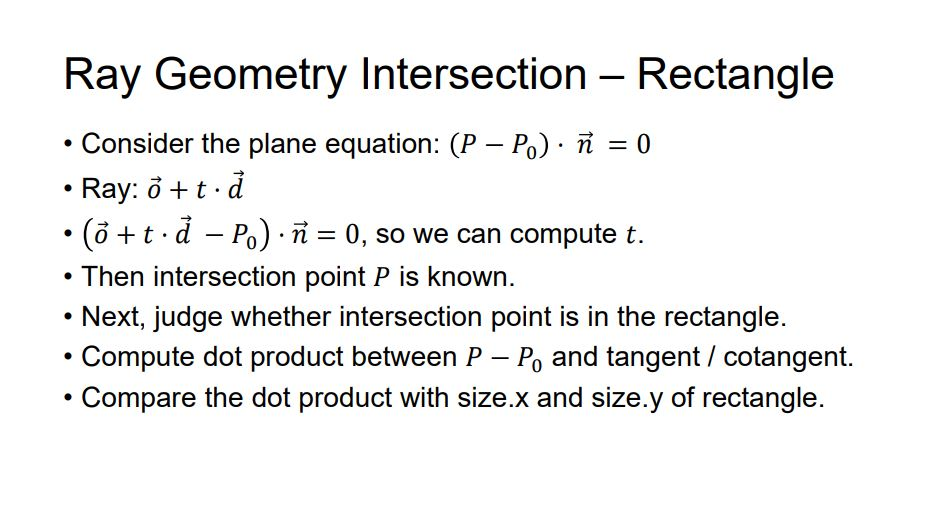
\includegraphics[width=8cm]{r1.JPG}}	
\end{figure}

As for ellipsoid, it seems hard. However, the process for sphere is easy.
Therefore, our basic idea is to do matrix transformation to simplify the problem to ray-sphere interseciton problem. 
The concrete steps are below.

\begin{figure}[h]
	\centering
	{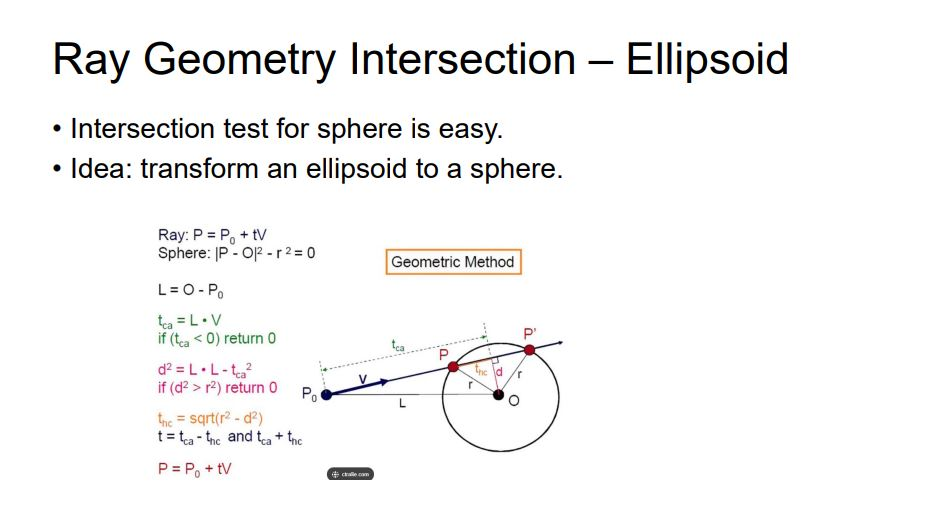
\includegraphics[width=8cm]{e1.JPG}}	
\end{figure}


\begin{figure}[h]
	\centering
	{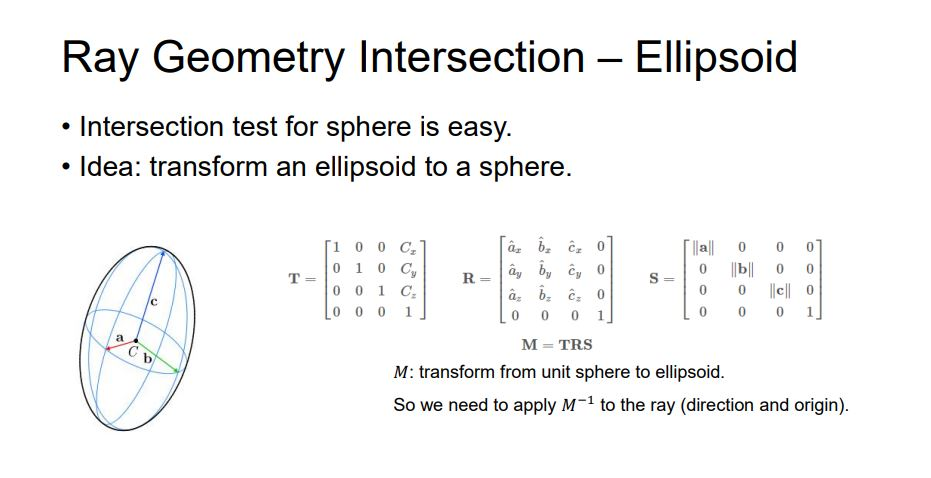
\includegraphics[width=8cm]{e2.JPG}}	
\end{figure}


\subsection{Phong Lighting at Intersection(Evaluate Radiance)}
\quad This part is implemented in the "integrator.cpp". We need to evaluate radiance using Phong lighting model.
In concrete, we should calculate the ambient, diffuse and specular at interseciton.


Ambient light comes from the environment. It is easy to calculate.


As for diffuse, we have to calculate dot product of light direction vector and normal vector, and multiply it with ligth\_color to get diffuse light.


As for specular, we first use math knowledge to calculate the reflected light direction vector. Also, we need to calculate the view direction vector. 
The next step is to calculate the dot product between the view direction and the reflect direction (it's non-negative) and then raise it to the shininess value of the highlight.
Next step is to multiply this with light color and a specular intensity value to get specular light.


At last, we sum them up.

\subsection{Direct Ray Tracing and Light Ray Sampling}
\quad This part is implemented in the function render() in "integrator.cpp".
If the ray first intersects with the LIGHT, then the radiance is the light color.
If the ray first intersects with the GEOMETRY, we need to generate a new ray which comes from the intersection postion to the light position. 
If the generated ray intersects with the GEOMETRY, then it is shadowed. We just need to calculat the ambient light. 
Otherwise, the radiance is set to the return value of radiance() function which is based on phong lighting model.


We have square area light, so we need to sample points from the rectangle. 
Therefore, different from point light, we can render the soft shadow effect by calculating the mean value. 
This soft shadow effect is illustrated in the picture below.
\begin{figure}[h]
	\centering
	{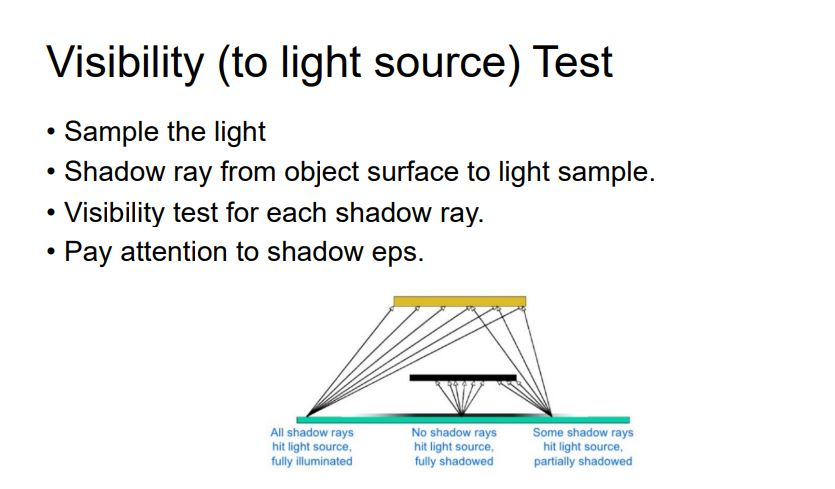
\includegraphics[width=8cm]{v1.JPG}}	
\end{figure}

\subsection{Anti-aliasing by Super-resolution}
\quad This part is implemented in sample\_pixel\_uniform() function in "camera.cpp".
I do the super resolution, which means I sample many points in each single pixel. The easiest way to do this is to take sample uniformly.
Furthermore, I apply some small tricks on it to get better effect, using the magic angle 26.6f. I do some rotations on the uniform samples. See more 
information in section "Advanced anti\_aliasing". 

\subsection{Texturing}
\quad This part is implemented most in the "texture.cpp", some in the "material.cpp" and "geometry.cpp".

The basic idea for texturing is mapping. In geometry.cpp, I need to add information in interaction.uv when doing the intersection. 
I just want to texture some rectangles, so I only modify the ray-rectangle intersection function. It is easy to get uv when we know the 2 direction dot product. 
The one thing to notice is that the uv would better be restricted to [0, 1]*[0, 1].


In "texture.cpp", the most important thing is to do the interpolation to get pixel value. I do the bilinear interpolation. 
I learn the knowledge about bilinear interpolation from the https://copyfuture.com/blogs-details/202112121313325372. 
The concrete algorithm is showed clearly in the picture below. 
\begin{figure}[h]
	\centering
	{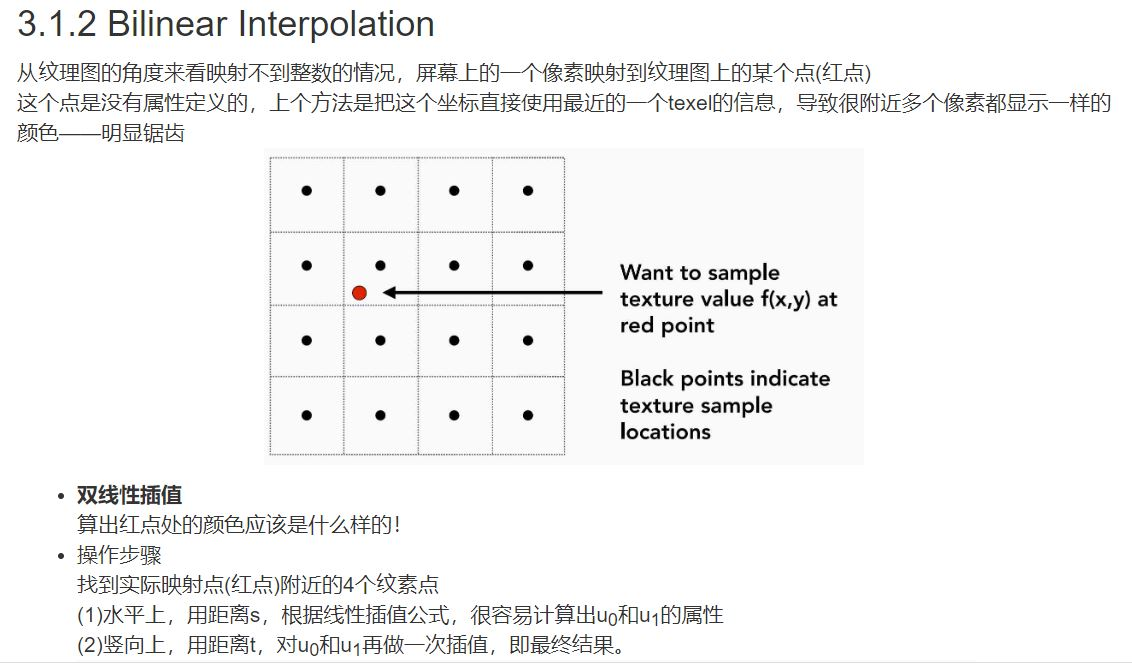
\includegraphics[width=8cm]{b1.JPG}}	
\end{figure}

\begin{figure}[h]
	\centering
	{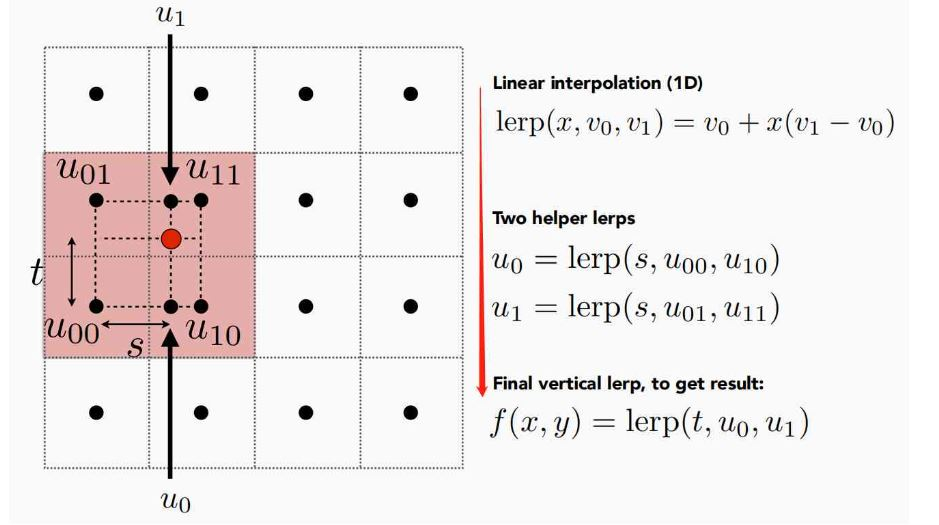
\includegraphics[width=8cm]{b2.JPG}}	
\end{figure}

In "material.cpp", we need to load textures and save them, specifying the type of them.(This step is to distinguish the normal texture and disp texture from basic texture.)


\subsection{Normal Texturing}
\quad This part is most implemented in the "geometry.cpp". 

For the basic texturing of a rectangle, the normals of texture are all the normal of the rectangle, 
which looks weird. If we use normal mapping, the normals of texture are given by the norm.jpg. 
However, these normals are not actually what we want, we need to do some transformation on them(aka normal mapping). 
The core code of normal mapping is given below.
\begin{lstlisting}	
	if(material->norm_t){
		Vec2f pos;
		Vec3f local_normal;
		pos = Vec2f(interaction.uv[0], interaction.uv[1]).cwiseProduct(Vec2f((float)material->norm_t->weight, (float)material->norm_t->height));
		local_normal = material->norm_t->get_tex_data((int)pos[1] + (int)pos[0] * material->norm_t->height);
		Vec3f final_normal = local_normal[2] * normal + local_normal[0] * tangent.normalized() + local_normal[1] * tangent.normalized().cross(normal.normalized());
		interaction.normal = final_normal.normalized();
    }
\end{lstlisting}

\subsection{Advanced Anti-aliasing}
\quad This part is implemented in sample\_pixel() function in "camera.cpp".
In section "Anti-aliasing", I take samples uniformly.
Furthermore, to get better effects, I apply some small tricks.


Firstly, I pick the samples randomly. However, there would be some hot/noise points! This isn't what I want. 
Therefore, I try to rotate the uniform samples using the magic angle 26.6f. 
I use the rotation matrix to multiply the samples and get points which are proper(not out of range). 
In this way, the effect of anti-aliasing seems better than the uniform sampling. 
The comparison can be seen in the result pictures.(I create a new scene where there is a ground made up of chess board, where the difference can be seen clearly)



\section{Results}
\quad Figure 2 is the Must part. Figure 3 is the Texturing. Figure 4 is Normal Texturing. Figure 5 is Anti-aliasing with Uniform Sampling. 
Figure 6 is Advanced Anti-aliasing by Rotating the uniform samples.
\begin{figure}[h]
	\centering
	{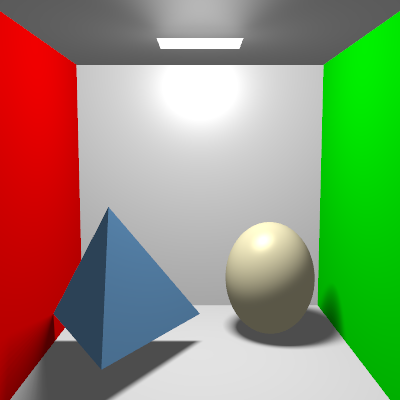
\includegraphics[width=8cm]{result1.png}}
	\caption{Basic ray tracing}	
\end{figure}

\begin{figure}[h]
	\centering
	{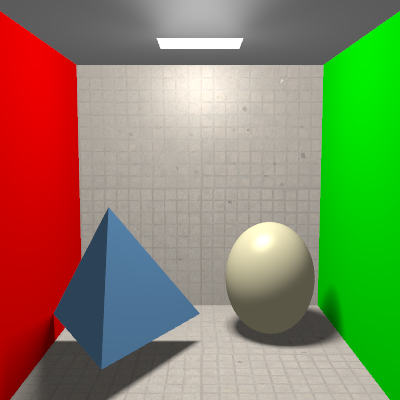
\includegraphics[width=8cm]{result_t.png}}	
	\caption{Texturing}
\end{figure}


\begin{figure}[h]
	\centering
	{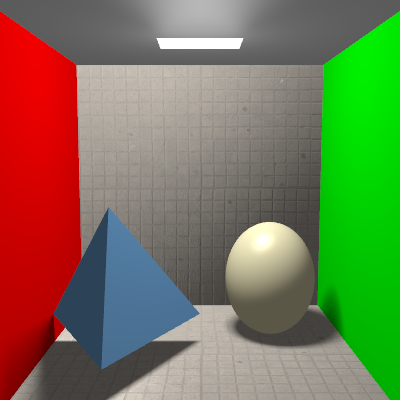
\includegraphics[width=8cm]{result_n.png}}
	\caption{Normal texturing}
\end{figure}

\begin{figure}[h]
	\centering
	{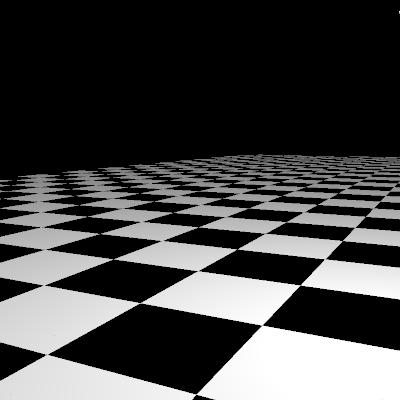
\includegraphics[width=8cm]{result_u.png}}
	\caption{Anti-aliasing with uniform sampling}
\end{figure}

\begin{figure}[h]
	\centering
	{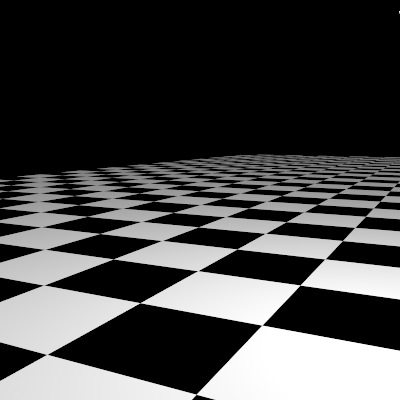
\includegraphics[width=8cm]{result_r.png}}
	\caption{Advanced anti-aliasing by rotating the uniform samples}
\end{figure}

\end{document}
